\section{Exercise 1: Assembly of the PDN netlist}

%%%%%%%%%%%%%%%%%%%%%%%%%%%%%%%%%%%%%%%%%%%%%%%%%%%%%%%%%%%

\subsection{Analysis of the provided models}

The PDN under analysis is described by three modules: the board, the package and the die. Before connecting them, the structure of each module has
been analysed, with particular attention to its ports, since these determine how the modules can be interconnected.

\begin{itemize}
    \item \textbf{Board}: The file \texttt{board\_passive.cir} contains the subcircuit \texttt{board\_passive}, a passive SPICE macromodel generated
    automatically by IdEM from the S-parameters of the board (\texttt{board.ts}) through a rational fitting over a 5~GHz bandwidth.\\ The model has two
    ports: port~1 is connected to the VRM, and port~2 to the package (VDD balls grouped together and GND balls grouped together). The model also
    accounts for the decoupling capacitors embedded in the board, for the parasitics of the VRM and for the other passive components of the board.
    \item \textbf{Package}: The file \texttt{package\_ports\_on\_caps\_passive.cir} contains the subcircuit\\
    \texttt{package\_ports\_on\_caps\_passive}, a macromodel of the same type obtained from the\\ S-parameters of the four-layer package
    (\texttt{package\_ports\_on\_caps.ts}).\\ It has seven ports: five ports placed on the locations of the decoupling capacitors
    (\texttt{VDD\_C01\_1}, \dots, \texttt{VDD\_C05\_1}), one port on the board side (the balls, with VDD and GND grouped) and one port on the die
    side (the bumps, with VDD and GND grouped). The ports on the capacitor locations make it possible to connect the decoupling capacitors externally,
    without modifying the package model.
    \item \textbf{Die}: The file \texttt{die\_model.sp} contains the subcircuit \texttt{die\_model}, which has two terminals, \texttt{vdd} and
    \texttt{vss}. Between them there are a current source, defined as a piecewise-linear (PWL) waveform, and an equivalent RC network
    (\texttt{passive\_network.sp.inc}) made of a 1~m$\Omega$ resistor in series with a 7~nF capacitor, which represents the parasitics of the power
    grid of the die. The PWL source models the noise generated by the switching activity of the device: it has 166\,664 points, spaced 72~ps apart,
    so that it lasts 12~$\mu$s, and its value ranges from about 21~mA to 287~mA.
\end{itemize}

\noindent All required modules have been included as follows:
\begin{lstlisting}[language={ltspice}, caption={Declaration of the modules in the netlist \texttt{pdn.cir}.}, label={lst:pdn_include}]
* Board macromodel:   ports (a_1,b_1)=VRM, (a_2,b_2)=package
.include "../input_files/board_passive.cir"

* Package macromodel: ports 1..5 = VDD_C01_1..VDD_C05_1, 6 = board, 7 = die
.include "../input_files/package_ports_on_caps_passive.cir"

* Die model: subckt die_model (vdd vss), PWL current load + RC power grid
.include "../input_files/die_model/die_model.sp"
\end{lstlisting}

\noindent\\ About \textbf{Port references}: the board and the package macromodels were generated with \textit{separate (floating)} port references:
each port $i$ is described by two terminals, the node $a_i$ associated to the port and the reference node $b_i$. For the models to be used in a
circuit simulation, the reference node of every port must be connected to the global ground.

%%%%%%%%%%%%%%%%%%%%%%%%%%%%%%%%%%%%%%%%%%%%%%%%%%%%%%%%%%%

\newpage
\subsection{Assembly of the complete netlist}

Then a new netlist has been created, \texttt{pdn.cir}, in which the files described above are included and properly connected, following the chain
VRM $\rightarrow$ board $\rightarrow$ package $\rightarrow$ die shown in \autoref{fig:pdn}.\\ The connections are the following:
\begin{itemize}
  \item the VRM is modelled simply as an ideal voltage source of 1~V (DC), connected to port~1 of the board;
  \item port~2 of the board is connected to the board-side port of the package;
  \item the die-side port of the package is connected to the supply terminal \texttt{vdd} of the die, which defines the node \texttt{vdie}, the die interface where the impedance and the voltage ripple are evaluated in the following exercises; the terminal \texttt{vss} of the die is connected to ground;
  \item the five ports of the package placed on the capacitor locations are brought out on the nodes \texttt{c01}, \dots, \texttt{c05} and left open, which corresponds to the PDN without decoupling capacitors; the capacitors will be connected between these nodes and ground in the following exercises;
  \item the reference node of all the ports is connected to the global ground (node~0).
\end{itemize}

\begin{figure}[!h]
\centering
 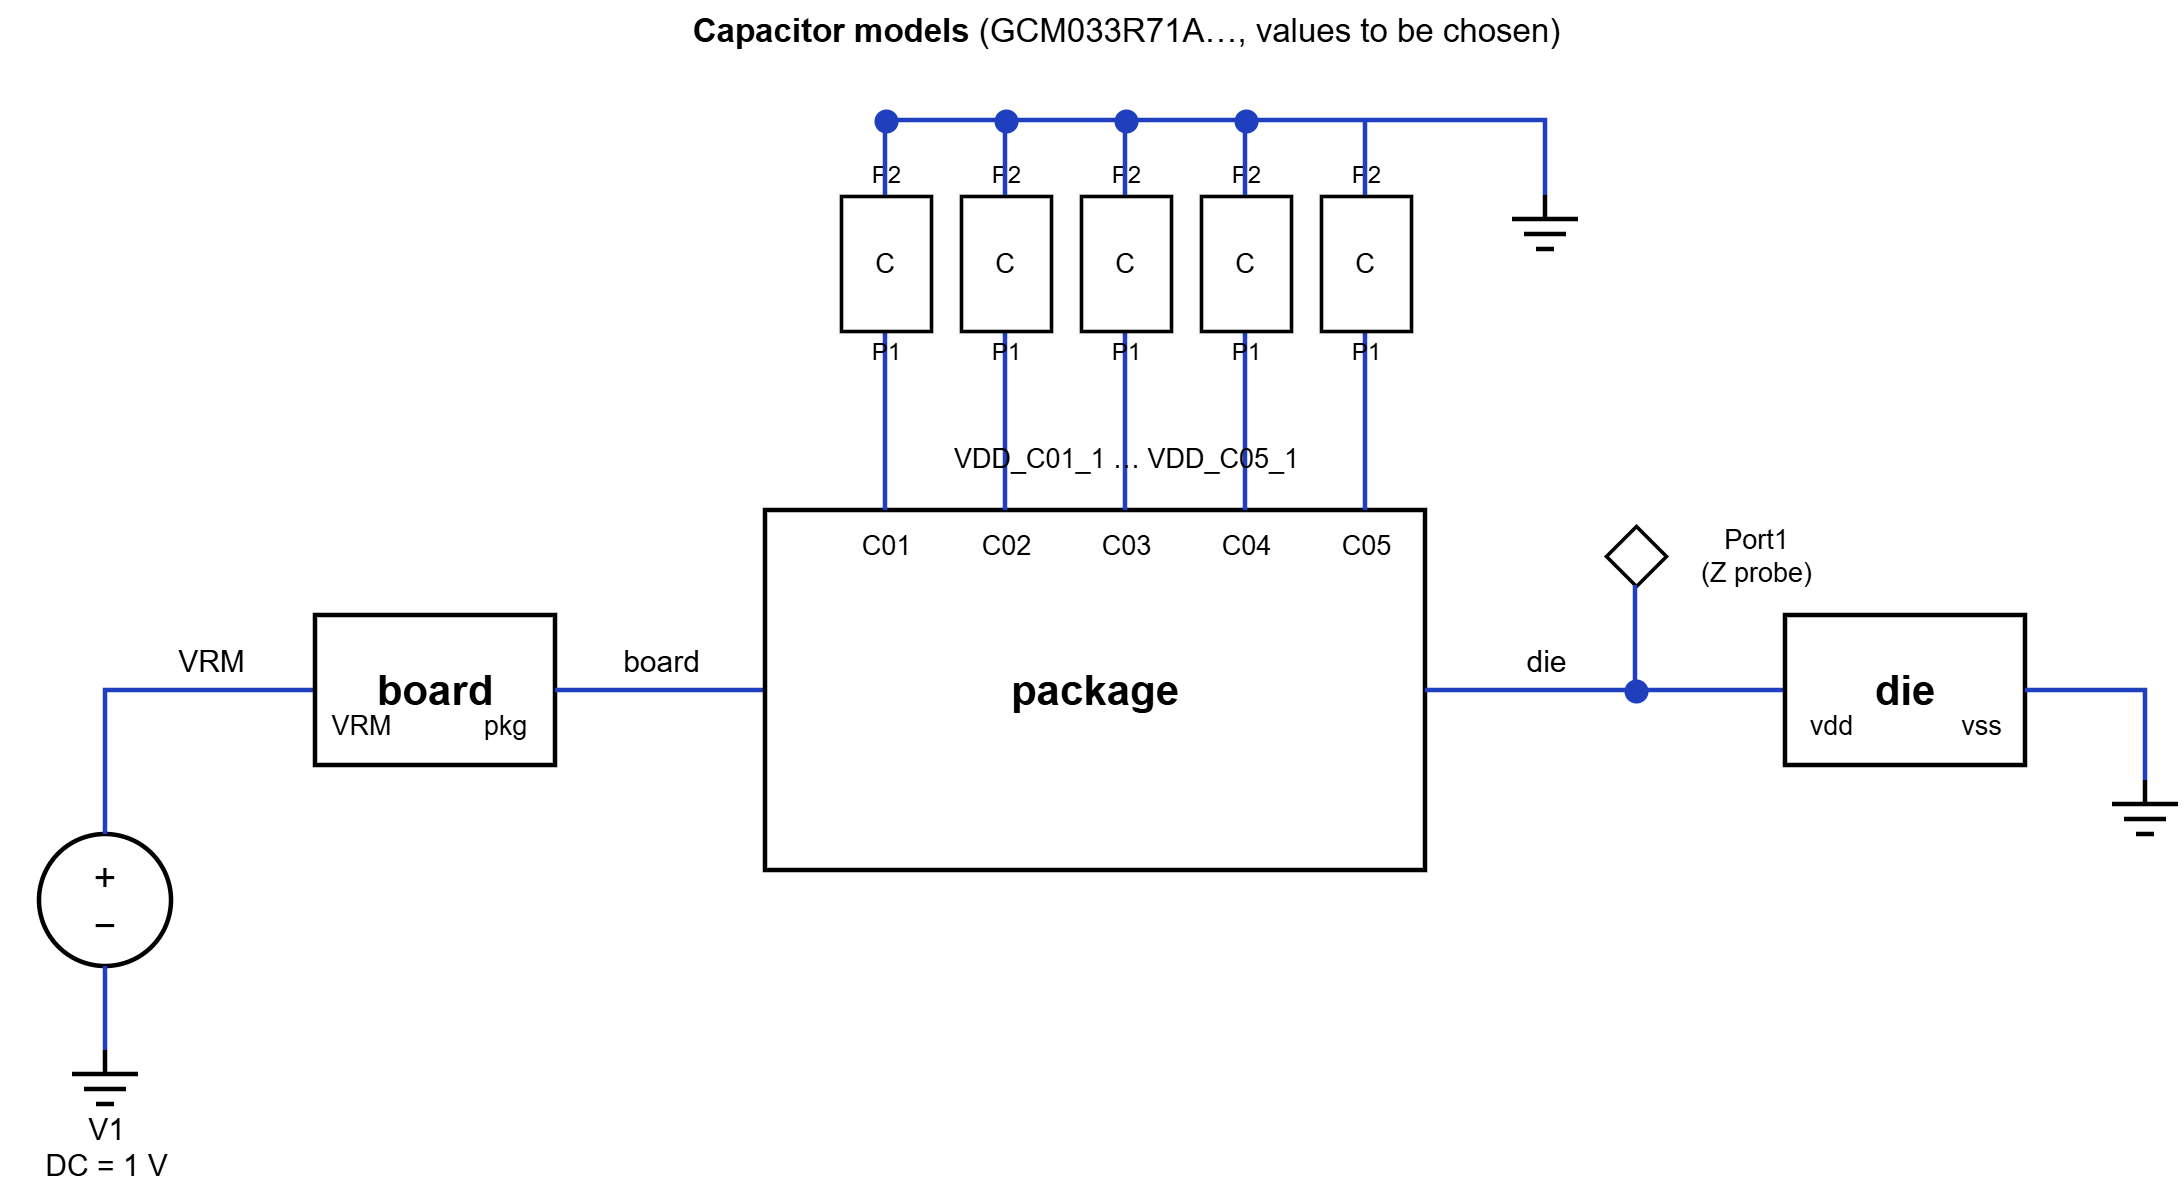
\includegraphics[width=0.95\textwidth]{./eser1/pdn_schematic.png}
\caption{Scheme of the complete PDN: ideal 1~V VRM, board, package and die. The five ports of the package on the capacitor locations (C01--C05) are left open in the PDN without decoupling capacitors.}
\label{fig:pdn}
\end{figure}

\noindent The part of the netlist that instantiates and connects the modules is shown in Listing~\ref{lst:pdn_inst}.

\begin{lstlisting}[language={ltspice}, caption={Instances and connection of the modules in the netlist \texttt{pdn.cir}.}, label={lst:pdn_inst}]
* ---- Supply: ideal VRM, 1 V DC ----
VVRM vrm 0 DC 1

* ---- Board: port 1 (VRM) on the source, port 2 (package) towards the package ----
* pin order: a_1 b_1 a_2 b_2
Xboard vrm 0 pkg_board 0 board_passive

* ---- Package ----
* pin order: a_1 b_1 ... a_7 b_7
*   1..5 = capacitor locations C01..C05
*   6    = board side (connected to board port 2)
*   7    = die side   (vdie)
Xpkg c01 0 c02 0 c03 0 c04 0 c05 0 pkg_board 0 vdie 0 package_ports_on_caps_passive

* ---- Die: VDD on node vdie, VSS on ground ----
Xdie vdie 0 die_model
\end{lstlisting}
